\documentclass{article}
\usepackage{graphicx} % Required for inserting images
\usepackage{wrapfig}
\usepackage{amsmath,amssymb,amsthm}
\usepackage{physics}
\usepackage{graphicx,float}
\graphicspath{{images/}}
\usepackage[none]{hyphenat}
\usepackage{blindtext}
\usepackage{parskip}
\usepackage[letterpaper,top=3cm, left= 3cm,bottom=3cm]{geometry}
\usepackage{subcaption}
\usepackage{tikz}
\usepackage{pgfplots}
\usepackage{esint}
\pgfplotsset{compat=1.18}
\usetikzlibrary{positioning,calc,patterns,angles,quotes,shapes,plotmarks}
\numberwithin{equation}{section}

\title{Electromagnetism}
\author{Polaris}
\date{2025/08/10}

\begin{document}

\maketitle
\newpage

\tableofcontents

\newpage
\section{Coulomb Force, Electric Field and more}
    \subsection{Coulomb Force}
        Coulomb Force is the equivalent of gravity in electromagnetism
        \begin{equation}
            \boxed{F_c = \frac{1}{4\pi \varepsilon_0} \frac{q_1 q_2}{r^2} = k_e \frac{q_1 q_2}{r^2}}
            \label{Coulomb Law}
        \end{equation}
        Where $\varepsilon_0$ is the vaccum electric permittivity, $k_e = 8.988 \cdot 10^9 \text{N}\cdot \text{m}^2 \cdot \text{C}^{-2}$ is the Coulomb constant, $q$ is the charge of the object and $r$ is the distance between them.

        In vector form, the force turns into 
        \[
        \vec{F_c} = \frac{1}{4\pi\varepsilon_0} \frac{q_1 q_2}{r^3} \vec{r} = \frac{1}{4\pi\varepsilon_0} \frac{q_1 q_2}{r^2}\hat{r}
        \]

    \subsection{Practice Problems}
        \subsubsection{Coulomb Force generated by a Semi Circle}
        Consider a half circle with a total charge of $Q_1$, a charge of $q_1$ is in the center of the circle, what is the force experienced by the charge in the center?
            \begin{figure}[H]
                \centering
                \includegraphics[width = 7cm]{pics/halfRingForce.png}
            \end{figure}

            It is not hard to see that the $y$ component of the Coulomb force is cancelled out.
            \[
            \Delta f = \frac{kq_1 \Delta q}{r^2} \cos \theta = \frac{kq_1 \lambda \Delta l}{r^2} \cos \theta
            \]
            Where $\Delta q = \lambda \Delta l$, $\lambda$ is the linear charge density, notice that $\Delta y = \Delta l \cos \theta$, therefore the total force is 
            \[
            \sum \Delta f = \sum \frac{kq_1 \lambda \Delta y}{r^2} 
            \]
            Therefore the force experienced by $q_1$ is 
            \begin{equation}
                F = F_0 2r = \frac{2r kq_1 Q_1}{\pi r r^2} = \frac{2k}{\pi} \frac{q_1 Q_1}{r^2}
                \label{Force of semi circle}    
            \end{equation}
            Where $F_0$ is the force exerted by a unit arc.

            \subsubsection{Coulomb Force generated by a Semi Sphere}
            Consider a half sphere with a total charge of $Q_2$, a charge of $q_2$ is in the center of the sphere, what is the force experienced by the charge in the center?
            \begin{figure}[H]
                \centering
                \includegraphics[width = 7cm]{pics/halfSphereForce.png}
            \end{figure}
            It is not hard to see force only points towards $y$ direction, the net force is $\Delta F_y = \Delta F \cos \theta$
    
            Denote surface charge density as $\sigma$, thus the force applied by a small surface element is 
            \[
            \Delta F_y = \frac{kq_2 \sigma \Delta S\cos \theta}{r^2}
            \]
            Thus the net force is 
            \[
            F_y = \frac{kq_2 \sigma}{r^2}\sum \Delta S \cos \theta
            \]
            $\Delta S \cos \theta$ is the projection of $\Delta S$ on the $x$ plane, therefore the summation gives the area of the largest circle of the sphere $\pi r^2$
            \begin{equation}
                F_{net} = F_0 \pi r^2 = \frac{k q_2 \sigma}{r^2} \pi r^2 = \frac{k}{2} \frac{Q_2q_2}{R^2_2} 
            \end{equation}
            Where $F_{net}$ is the force exerted by a small surface element
    \subsection{Electric Field}
        Electric field is defined as
        \begin{equation}
            \boxed{\vec{E} = \frac{\vec{F}}{q}}
            \label{E field}
        \end{equation}

        In other words, the electric field experience by a test charge at a position is equal to the force it experience divided by the charge of the object.

        This test charge must satisfy 2 requirements:
        \begin{enumerate}
            \item It is small enough to be treated as a point 
            \item The charge is small enough to not disrupt the overall electric field distribution
        \end{enumerate}

    \subsubsection{Field Line}
        Field line is a way to visualize electric field, the lines satisfy 2 reqiurements:
        \begin{enumerate}
            \item The direction of arrow indicates the direction of the force that a positive charge experience
            \item The density (how many lines per unit area/volume) is proportional to the magnitude of electric field
        \end{enumerate}

        \begin{figure}[H]
            \includegraphics[width=10cm]{pics/field_line.png}
            \centering
            \caption{Electric field line of a positive charge and a negative charge}
        \end{figure}

        If there are more than one electric field present in a region, the net electric field is 
        \begin{equation}
            \vec{E}_{net} = \sum_{i=1}^{n} \vec{E}_i
            \label{Adding E field}
        \end{equation}

        \subsubsection{Gauss Law}
        The integral form of Gauss law is in the form of (this is equivalent to Coulomb's Law)
        \begin{equation}
            \boxed{\oiint \vec{E} \cdot d\vec{A} = \frac{1}{\varepsilon_0} \sum q}
            \label{Gauss Law}
        \end{equation}
        The LHS of the equation is also known as the electric flux $\phi_E$, it measures how many electric field lines go through a certain area.

    \subsection{Practice Problems}
        \subsubsection{Electric Field of a infinite sheet}
            Consider an infinite sheet with a surface charge density of $\sigma$, find the electric field strength of this object (assume $\sigma >0$)

            It is not hard to see that electric field is perpendicular to the sheet, because both $x$ and $y$ direction cancel each other out.

            \begin{figure}[H]
                \includegraphics[width=10cm]{pics/sheet_field.png}
                \centering
                \caption{Electric field of a sheet}
            \end{figure}

            There are 3 Gaussian surface in this cylinder, 2 circles and 1 side, on the side there is no electric flux because no field line goes through it. On the top and bottom, electric field line goes through this surface perpendicularly, therefore
            \[
            \phi_E = E \int dA = E A
            \]
            The total electric flux is 

            \[
            \oiint \vec{E} \cdot d\vec{A} = EA + EA = 2EA
            \]

            By Gauss Law:
            \[
            2EA = \frac{\sum q}{\varepsilon_0}
            \]
            By the definition of charge density $\sum q = \sigma A$, the electric field is thus
            \begin{equation}
                E = \frac{\sigma}{2\varepsilon_0}
                \label{E field of sheet}
            \end{equation}

        \subsubsection{Electric Field of a conductor}
        2. Find the electric field as the surface of the conductor

        Draw a Gaussian surface similar to the situation above (this time the cylinder is very small so the enclose area is approxiamtely a flat plane)

        By Gauss Law:
        \[
        EA = \frac{\sum q}{\varepsilon_0}
        \]
        By the definition of charge density $\sum q = \sigma A$, the electric field is thus
        \begin{equation}
            E = \frac{\sigma}{\varepsilon_0}
            \label{E field of conductor surface}
        \end{equation}

        There are 2 property of static electric field of a metal conductor
        \begin{enumerate}
            \item There is no electric field and charge inside the conductor (otherwise there will be a current inside the conductor)
            \item The electric field on the surface is perpendicular to the surface (ptherwise the component that is not perpendicular to the surface will cause charge to move)
        \end{enumerate}

        \subsubsection{Electric Field of shell conductor}
        Consider a shell conductor with a charge of $Q_1$, inner radius of $r_1$ and outer radius of $r_2$ there is a charge $Q_2$ located at the center of the conductor, find the distribution of $E$.

        \textbf{Solution: }There are $3$ region separarted by the shell, $0<r<r_1$ (the volume inside the inner circle), $r_1 < r < r_2$ (the volume inside the shell), $r>r_2$ (the area outside the shell), we need to consider them separartely.

        \begin{enumerate}
            \item $0<r<r_1$, draw a Guassian surface (dotted circle) as such
            \begin{center}
                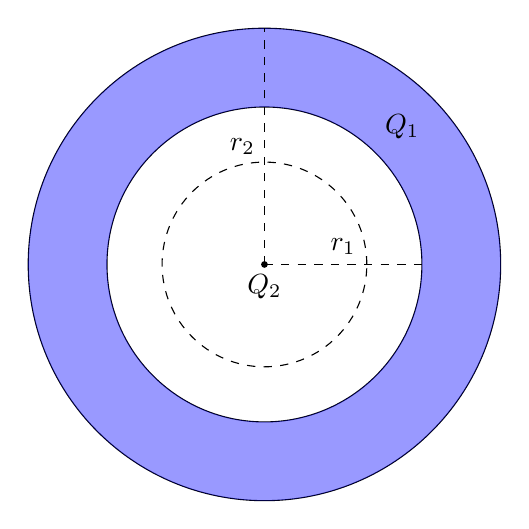
\begin{tikzpicture} 
                    \draw (0,0) circle (3cm);
                    \draw (0,0) circle (2cm);
                    \draw[dashed] (0,0) circle (1.3cm);
                    \fill[blue, fill opacity=0.4, even odd rule] (0,0) circle (3cm) (0,0) circle (2cm);
                    \draw (0,0)[dashed] -- (2,0) node [midway,above] {$r_1$};
                    \draw (0,0)[dashed] -- (0,3) node[midway,left] {$r_2$};
                    \draw[fill=black] (0,0) circle (1pt) node[below]{$Q_2$};
                    \draw(1.75,1.75) node {$Q_1$};
                \end{tikzpicture}
            \end{center}
            By Gauss Law
            \begin{align*}
                E \cdot4\pi r^2 = \frac{1}{\varepsilon_0}Q_2\\
                E = \frac{1}{4\pi \varepsilon_0} \frac{Q_2}{r^2} = \frac{k_e Q_2}{r^2}
            \end{align*}

            \item $r_1 < r < r_2$, this region is within the conductor, meaning there is no electric field in this region ($E=0$)

            \item $r > r_2$, draw a Gaussian surface (dotted circle) as such
            \begin{center}
                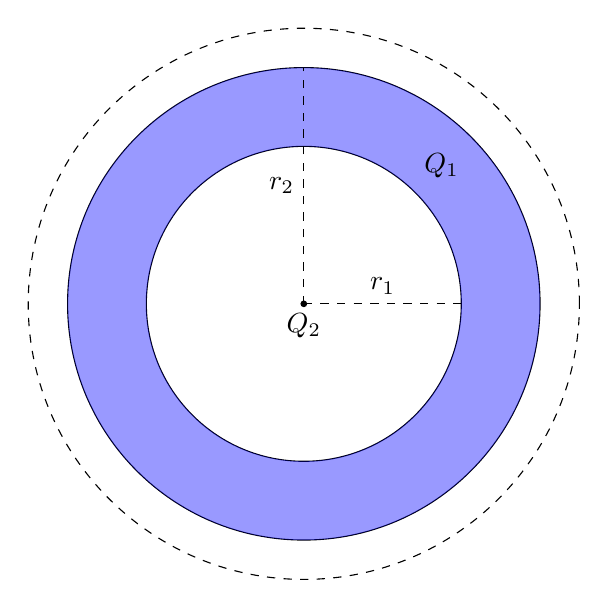
\begin{tikzpicture} 
                    \draw (0,0) circle (3cm);
                    \draw (0,0) circle (2cm);
                    \draw[dashed] (0,0) circle (3.5cm);
                    \fill[blue, fill opacity=0.4, even odd rule] (0,0) circle (3cm) (0,0) circle (2cm);
                    \draw (0,0)[dashed] -- (2,0) node [midway,above] {$r_1$};
                    \draw (0,0)[dashed] -- (0,3) node[midway,left] {$r_2$};
                    \draw[fill=black] (0,0) circle (1pt) node[below]{$Q_2$};
                    \draw(1.75,1.75) node {$Q_1$};
                \end{tikzpicture}
            \end{center}
            By Gauss Law
            \begin{align*}
                E \cdot4\pi r^2 = \frac{1}{\varepsilon_0}(Q_2+Q_1)\\
                E = \frac{1}{4\pi \varepsilon_0} \frac{Q_2+Q_1}{r^2} = \frac{k_e (Q_2+Q_1)}{r^2}
            \end{align*}
        \end{enumerate}

        \subsubsection{Electric Field of a Infinite Line}
        Consider a line with a linear charge density of $\lambda$, what is the electric field around this line?

        It is not hard to see that electric field is perpendicular to the line because the component parallel to the line is cancelled.

        There are 3 approaches to this problem 
        \begin{enumerate}
            \item Integral approach, consider such line
            \begin{center}
                \begin{tikzpicture}
                    \coordinate (A) at (0,2.5);  % 顶点O
                    \coordinate (B) at (3,0);    % 角的一边
                    \coordinate (C) at (3.5,0);    % 角的另一边(水平线上的点)
                    \coordinate (P) at (-5,0);
                    \coordinate (Q) at (5,0);
                    \coordinate(O) at (0,0);
                    \coordinate (H) at ($(A)!(B)!(C)$);
                    
                    \draw (P) -- (Q);
                    \draw[fill=black] (A) circle (1pt) node[above]{$O$};
                    \draw (A) -- (B) node[midway,below]{$r$};
                    \draw[dashed] (A) -- (C) node[midway,above]{$r$};

                    \draw (A) -- ($(P)!(A)!(Q)$) node[midway, left]{$r_0$};
                    \draw[dashed] (B) -- ($(A)!(B)!(C)$);
                    
                    \pic [draw, angle radius=30mm, angle eccentricity=1.1, "$d\theta$"] {angle = B--A--C};
                    \pic [draw, angle radius=2mm, angle eccentricity=1.1] {right angle = A--O--Q};
                    \pic [draw, angle radius=6mm, angle eccentricity=1.3, "$\theta$"] {angle = O--A--B};
                    \pic [draw, angle radius = 1mm, angle eccentricity = 1.1, "$\theta$" below] {angle = C--B--H};
                \end{tikzpicture}
            \end{center}
            The length of the line segment is $dl = \dfrac{rd \theta}{\cos \theta} = \dfrac{r_0 d\theta}{\cos^2 \theta}$, thus the charge of this segment is $dq = \dfrac{\lambda r_0 d\theta}{\cos^2 \theta}$, the distance to the line segment is $r = \dfrac{r_0}{\cos \theta}$, the electric field is thus
            \begin{align*}
                dE &= \frac{kdq}{r^2}\cos\theta \\
                E &= 2\int_{0}^{\frac{\pi}{2}} \frac{k \lambda r_0}{\cos^2 \theta} \frac{\cos^2 \theta}{r^2_0} \cos\theta\\
                &= \frac{2\lambda}{4\pi \varepsilon_0 r_0} \int_{0}^{\frac{\pi}{2}} \cos \theta d\theta\\
                &= \frac{\lambda}{2\pi\varepsilon_0 r_0}
            \end{align*}

            \item Using Gauss Law, draw a cylinder Gaussian surface as such (the side of the cylinder is not drawn)
            \begin{center}
                \begin{tikzpicture}
                    \coordinate (A) at (-5,0);
                    \coordinate (B) at (5,0);
                    \coordinate (O) at (0,1);

                    \draw (A) -- (B);
                    \draw[fill=black] (O) circle (1pt) node[above]{$O$};
                    \draw[dashed] (-5,1) -- (5,1);
                    \draw[dashed] (-5,-1) -- (5,-1);

                    \draw (O) -- ($(A)!(O)!(B)$) node[midway,left]{$r_0$};
                \end{tikzpicture}
            \end{center}
            The area of the cylinder where there is an electric flux is $A = 2\pi r_0 h$, where $h$ is the length of the cylinder, the charge of the cylinder is $q_{tot} = \lambda h$, thus
            \[
            E \cdot 2\pi r_0 h = \frac{1}{\varepsilon_0} q_{tot}
            \]
            \begin{equation}
                E = \frac{\lambda}{2\pi \varepsilon_0 r_0}
                \label{E field of line}
            \end{equation}

            \item Consider a circle that is positioned as such 
            \begin{center}
                \begin{tikzpicture}
                    \coordinate (A) at (0,2.5);  % 顶点O
                    \coordinate (B) at (3,0);    % 角的一边
                    \coordinate (C) at (3.5,0);    % 角的另一边(水平线上的点)
                    \coordinate (P) at (-5,0);
                    \coordinate (Q) at (5,0);
                    \coordinate(O) at (0,0);
                    \coordinate (H) at ($(A)!(B)!(C)$);
                    
                    \draw (P) -- (Q);
                    \draw[fill=black] (A) circle (1pt) node[above]{$O$};
                    \draw (A) -- (B) node[midway,below]{$r$};
                    \draw[dashed] (A) -- (C);
                    \draw (3.4,0) node [below] {$\Delta l$};

                    \draw (A) -- ($(P)!(A)!(Q)$) node[midway, left]{$r_0$};
                    \draw[dashed] (B) -- ($(A)!(B)!(C)$) node [above]{$\Delta l_2$};
                    \draw (2.9, 1.32) node [left] {$\Delta l_1$};
                    
                    \pic [draw, angle radius=2mm, angle eccentricity=1.1] {right angle = A--O--Q};
                    \pic [draw, angle radius=6mm, angle eccentricity=1.3, "$\theta$"] {angle = O--A--B};
                    \pic [draw, angle radius = 1mm, angle eccentricity = 1.1] {angle = C--B--H};

                    \draw (A) ++(-2.5,0) arc (180:360:2.5);

                    \end{tikzpicture}
            \end{center}
            The three line segment has a length of $\Delta l_1 = r_0 d\theta$, $\Delta l_2 = r d\theta$, $\Delta l = \dfrac{\Delta l_2}{\cos \theta}$, therefore
            \[
            \frac{\Delta l_1}{r_0} = \frac{\Delta l_2}{r}
            \]
            The electric field generated by $\Delta l$ is 
            \[
            \Delta E = \frac{k \lambda \Delta l }{r^2} = \frac{k \lambda }{r^2} \frac{\Delta l_2}{\cos \theta} = \frac{k\lambda}{r^2} \frac{r \Delta l_1}{r_0 \cos\theta}
            \]
            Notice that $r\cos \theta = r_0$
            \[
            \Delta E = \frac{k\lambda \Delta l_1}{r_0^2}
            \]
            This means that the infinite line creates a equal electric field compared to the half circle. The electric field generated is thus
            \begin{align*}
                E = \frac{F}{q_0} = \frac{F_0}{q_0} 2r_0 = \frac{kq_0 \lambda 2r_0}{q_0 r_0^2} = \frac{2k\lambda}{r_0} = \frac{\lambda}{2\pi \varepsilon_0 r_0}
            \end{align*}
        \end{enumerate}

        \newpage
        \section{Direct Current Circuit}
        Define \textbf{voltage} (unit: V) as the potential difference between two points in the circuit
        \begin{equation}
            V = \frac{W}{q}
        \end{equation}
        Where $W$ is the work done to the electric current, the voltage of the battery is called electromotive force (denote as $\varepsilon$, emf for short), a voltage difference drives the electron to flow.

        Define \textbf{current} (unit: A) as the amount of charge that flows through a certain point over a period of time
        \begin{equation}
           I = \frac{dQ}{dt}
        \end{equation}
        Since current is made up of electron, the following expression can be written
        \[
        I = \frac{dQ}{dt} = \frac{Ne}{\Delta t} = \frac{n\Delta A v e \Delta t}{\Delta t} = n\Delta A ve
        \]
        Where $\Delta A$ is the cross section area of the wire, $e$ is the elementary charge, $n$ is the number density of electron, $v\Delta t$ is the distance travelled by the electron over a period of time, here $v$ is called the drift velocity (disregaring thermal motion), it is usually very slow ($10^{-3}$ m/s)
        \subsection{Resistor and Ohm's Law}
        Ohm's Law measures the resistance $R$ (unit: $\Omega$) of a electrical component
        \begin{equation}
            R = \frac{V}{I}
        \end{equation}
        Where $I$ is the current through the component, larger the resistance, harder the electron will flow through this component.
        \begin{figure}[H]
            \centering
            \includegraphics[width=3cm]{pics/resistor.png}
            \caption{Symbol for resistor}
        \end{figure}
        \subsubsection{Diode}
        Diode is a special electrical component, it only allows current to flow through one way, from anode to cathode.
        \begin{figure}[H]
            \centering
            \includegraphics[width=3cm]{pics/diode.png}
            \caption{Symbol for diode}
        \end{figure}
        The V-I curve of diode looks like this
        \begin{figure}[H]
            \centering
            \includegraphics[width=10cm]{pics/diodeVIcurve.png}
            \caption{V-I graph of diode}
        \end{figure}
        Here $V_d$ is the minimum voltage it takes to drive a current through the diode, in the area in blue, diode stops the current from flowing the other way, and $V_{br}$ is the minimum energy it takes to penetrate the diode.
        
        \subsection{Parallel and Series}
        \begin{figure}[H]
            \centering
            \includegraphics[width=10cm]{pics/parallel_series.png}
            \caption{Series (left) and parallel (right)}
        \end{figure}
        For a series circuit, the current is the same for all loads in the circuit.
        \[
        \begin{cases}
            I = I_1 + I_2\\
            V = V_1 + V_2\\
        \end{cases}        
        \]
        For a parallel circuit, the voltage drop across all load is the same
        \[
        \begin{cases}
            I = I_1 + I_2\\
            V = V_1 = V_2\\
        \end{cases}        
        \]

        \subsubsection{Voltmeter and Ammeter}
        Voltmeter and ammeter are equipment that measures the voltage drop across a load and the current that flows through a load
        \begin{figure}[H]
            \centering
            \includegraphics[width=10cm]{pics/voltmeter_ammeter.png}
            \caption{Voltmeter(left) and ammeter(right)}
        \end{figure}
        \newpage
        \section{Magnetism}
        Magnetism studies magnets, it is closely related to electricity, in fact current produce magnetic field.

        \subsection{Magnetic Field}
        Magnetic field (denote as $B$) is the same as electric field, except it is defined for magnetic forces
        \begin{figure}[H]
            \centering
            \includegraphics[width=10cm]{pics/magneticLine.png}
            \caption{Magnetic field line of a magnet}
        \end{figure}
        Currently, no magnetic monopole is observed, therefore magnetic field line looks like a equivalent effect of a north and south pole.

        \subsection{Ampere's Law}
        Ampere's Law is the Gauss Law of magnetism, it points the relation between the current and its induced magnetic field
        \begin{equation}
            \boxed{\oint \vec{B} \cdot d\vec{L} = \mu_0 \sum I_{int}}
        \end{equation}
        Where $\mu_0 = 4\pi \cross 10^{-7}$ H/m is the vaccum permability, $I_{int}$ is the current through a enclosed surface. 
        
        Notice that if a current flows into a Ampere loop then flows out of it, there will be no magnetic field induced.
        
        The direction of magnetic field will be determined by Right Hand rule.
        \begin{figure}[H]
            \centering
            \includegraphics[width=8cm]{pics/RHR.png}
            \caption{Right Hand Rules}
        \end{figure}

        \subsubsection{Magnetic Field generated by a wire}
        \begin{figure}[H]
            \centering
            \includegraphics[width = 8cm]{pics/AmperesLaw1.jpg}
            \caption{Magnetic field generated by a wire}
        \end{figure}
        Consider a Ampere Loop that has a distance $r$ to the wire, therefore
        \[
        B\cdot L = \mu_0 I
        \]
        \begin{equation}
            B = \frac{\mu_0 I}{2\pi r}
            \label{BfieldWire}
        \end{equation}

        \subsubsection{Magnetic Field generated by a coil}
        Consider a coil with a uniform loop per unit length of $n = N/L$, a current of $I$ pass through this coil. The wire blocks the magnetic field of going outside the coil, therefore it is traped inside the coil shown in the figure below.
        \begin{figure}[H]
            \centering
            \includegraphics[width=8cm]{pics/BfieldCoil.png}
            \caption{Magnetic field generated by a coil}
        \end{figure}
        Consider a Ampere Loop shown in red, the current passed through is $I_{int} = NI$, where $N$ is the number of coil
        \[
        B L = \mu_0 N I
        \]
        \begin{equation}
            B = \mu_0 n I 
            \label{BfieldCoil}
        \end{equation}

        \subsubsection{Biot-Savart Law}
        Biot-Savart law shows the relation between a current element and the induced magnetic field element. (the direction of current is the direction of $d\vec{L}$)
        \begin{equation}
            d\vec{B} = \frac{\mu_0}{4\pi} \frac{I d\vec{L} \cross \vec{r}}{r^3}
        \end{equation}

        \begin{figure}[H]
            \centering
            \includegraphics[width=10cm]{pics/bsLaw.png}
            \caption{Biot Savart Law}
        \end{figure}

        \subsection{Lorentz Force}
        Lorentz force is a forced experienced by a particle moving through electric and magnetic field, however this section is only about magnetic field. The force experienced 
        \begin{equation}
            \boxed{\vec{F} = q (\vec{v}\cross \vec{B})}
            \label{Lorentz Force}
        \end{equation}
        \subsubsection{Lorentz Force on a rod}
        Consider a rod with a current through it, the electrons are moving at a speed of $v = \dfrac{\Delta x}{\Delta t}$, thus the force experience by each indivisual electron is 
        \[
        \Delta F = \frac{q}{\Delta t} B\Delta x
        \]
        Assume that there are a total of $N$ electrons flowing through the rod with a length of $l$, the total force experienced is thus
        \[
        F = \sum F = N l \frac{q}{\Delta t} B
        \]
        Here $\dfrac{Nq}{\Delta t}$ is the total current that flowed through the rod, thus the force experienced by a moving rod is 
        \begin{equation}
            \vec{F} = l(\vec{B} \cross \vec{I})
        \end{equation}
        Where $I$ is the current through the rod and $L$ is the length of the rod.
        
        \subsubsection{Cyclotron}
        Cyclotron is a machine used to acclerate particles
        \begin{figure}[H]
            \centering
            \includegraphics[width=10cm]{pics/cyclotron.png}
            \caption{Cyclotron}
        \end{figure}
        In the middle there is an electric field that cause the particle to accelerate, and the magnetic field turns the particle around. This is because a Lorentz force applied on a particle will cause it to undergo circular motion.
        \[
        qvB = m \frac{v^2}{R}
        \]
        Therefore the period of the particle is 
        \[
        T = \frac{2\pi m}{qB}
        \]
        If the alternating current has the same period as the particle, then the particle will always accelerate when it pass through the area with electric field.

        The disadvantage of cyclotron is after the velocity of the particle reached a very high velocity, relativistic effects comes in and cause the mass to change, thus the period, then AC source will have difficulties to match the motion of particle.
        
        \subsubsection{Cyclotron Problems}
        Consider a cyclotron with a radius of $R$, a magnetic field strength of $B$, the maximum voltage of AC is $\varepsilon$ the accelerated particle has a mass of $m$ and charge of $q$, find
        \begin{enumerate}
            \item the time spent in magnetic field
            \item The time spent in electric field
        \end{enumerate}

        1. Everytime, the particle experience a constant gain of kinetic energy of $K = q\varepsilon$, the final kinetic energy is
        \[
        K_f = \frac{1}{2} m \left(\frac{qBR}{m}\right)^2 = \frac{q^2 B^2 R^2}{2m}
        \]
        The final velocity is founded by equating Lorentz force and centrifugal force when the particle is exiting the cyclotron.

        Assumes it takes $N$ cycle to achieve this final energy.
        \[
        N = \frac{K_f}{K} = \frac{q^2B^2R^2}{2q m\varepsilon} = \frac{qB^2 R^2}{2m\varepsilon}
        \]
        Therefore the time spent in magnetic field is
        
        \[
        t_m = N \cdot T = \frac{qB^2R^2}{2m\varepsilon} \cdot \frac{2\pi m}{qB} = \frac{\pi qB R^2}{\varepsilon}
        \]

        2. In electric field, the particle is undergoing accelerating motion $v_f = at$, $a$ is the acceleration, which can be given by Newton's Second Law
        \[
        a = \frac{qE}{m}
        \]
        Thus 
        \[
        t_E = \frac{v_f}{a} = \frac{q^2B^2R^2}{m^2} \frac{m}{qE} = \frac{qB^2R^2}{qmE}
        \]

        \subsection{Faraday's Law of Induction}
        Michael Faraday discovered that moving a coil through a area with a nonzero magnetic field strength, an induced emf will be generated, the induced emf is given by
        \begin{equation}
            \boxed{\varepsilon = -N\frac{\Delta \Phi_B}{\Delta t}}
            \label{Faraday Law}
        \end{equation}

        Where $\Delta \phi_B = \vec{B} \cdot \vec{A}$ is the magnetic flux of a region, $N$ is the number of coils.
        
        \subsubsection{Lenz's Law}
        The negative sign in Faraday's Law is known as the Lenz's Law, it stated that magnetic flux tend to stay constant, therefore it will resist the change of current through the induced emf.

        \subsection{Inductor}
        The most simple inductor is a coil, due to Faraday's Law, when an alternating current pass through, a induced emf will be generated
        \begin{align*}
            \varepsilon &= -N \frac{\Delta \phi_B}{\Delta t}\\
            &= -N A \frac{\Delta B}{\Delta t}\\
            &= -N A \frac{\Delta (\mu_0 n I)}{\Delta t}\\
            &= -N A \mu_0 n \frac{dI}{dt}
        \end{align*}
        Where $n$ is the number of coil in unit length, define \textbf{inductance} $L = N A \mu_0 n$, when an AC pass through an inductor, it will generate a emf of
        \begin{equation}
            \boxed{\varepsilon = -L \frac{dI}{dt}}
            \label{inductance}
        \end{equation}
        The unit of inductance is H(enry).
        
        \subsubsection{Energy Stored by an Inductor}
        Energy is defined as 
        \[
        E = \int V I dt
        \]
        Where $V = L \dfrac{dI}{dt}$, therefore the energy stored is
        \begin{equation}
            \boxed{E = \frac{1}{2}L I^2}
        \end{equation}

        \subsection{Circuits with Inductor}
        \subsubsection{Inductor and Resistor}
        There are two types of LR circuit, with battery and without battery, first take a look at a LR circuit without battery. A LR circuit with battery is similar to a RC discharging circuit.

        \begin{figure}[H]
            \centering
            \includegraphics[width=8cm]{pics/LRnoBattery.png}
            \caption{LR circuit without battery}
        \end{figure}

        Assume that there is an initial current of $I_0$ flowing through the current, by Kirchhoff's 2nd Law
        \[
        -IR - L \frac{dI}{dt} = 0
        \]
        This differential equation results to an exponetial function
        \begin{equation}
            I = I_0 e^{-(t/\tau)}
            \label{LR no battery}
        \end{equation}
        Where $\tau = \dfrac{L}{R}$ is the time constant of this circuit, just like RC circuit.

        A LR circuit with battery is similar to an RC charging circuit, consider the following circuit, the battery provides an emf of $\varepsilon = \varepsilon_0 \sin(\omega t +\phi_0)$

        \begin{figure}[H]
            \centering
            \includegraphics[width=8cm]{pics/LRwBattery.png}
            \caption{LR circuit with battery}
        \end{figure}
        By Kirchhoff's 2nd law
        \[
        \varepsilon - L\frac{dI}{dt} - IR = 0
        \]
        This differential equation also results in an exponetial function
        \begin{equation}
            I = I_0 \left(1-e^{(-(t/\tau))}\right)
            \label{LR battery}
        \end{equation}
        Where $I_0$ is the current after the whole circuit is stable, $I_0 = \dfrac{\varepsilon}{R}$.

        In the figure below, $x$ axis is time and $y$ axis is current.
        \begin{figure}[H]
            \centering
            \includegraphics[width=10cm]{pics/LRgraph.png}
            \caption{Relation of current and time in an LR circuit}
        \end{figure}

        \subsubsection{Inductor and Capacitor}
        \begin{figure}[H]
            \centering
            \includegraphics[width=8cm]{pics/LCnoBattery.png}
            \caption{LC circuit without battery}
        \end{figure}
        Assume the capacitor is fully charge, by Kirchhoff 2nd Law
        \[
        \frac{Q}{C} - L \frac{dI}{dt} = 0
        \]
        Where $I = -\dfrac{dQ}{dt}$, substitute this in, it results in a differential equation
        \[
        \frac{I}{C} + L\frac{d^2I}{dt^2} = 0
        \]
        This is a differential equation of SHM, the solution is 
        \begin{equation}
            I = I_0 \cos(\omega t + \phi_0)
            \label{current RC without battery}
        \end{equation}
        \begin{equation}
            Q = Q_0 \sin(\omega t+\phi_0)
            \label{charge RC without battery}
        \end{equation}
        Where $\omega = \sqrt{\dfrac{1}{LC}}$, $I_0 = \omega Q_0$ is the peak current through this circuit. The oscillation period of this circuit is $P = 2\pi \sqrt{LC}$
        
        A LC circuit with a battery is not possible because without a resistor, the current will explode to infinity when the battery is connected.

        \subsubsection{Resistor, Capacitor and Inductor}
        \begin{figure}[H]
            \centering
            \includegraphics[width=8cm]{pics/LRCnoBattery.png}
            \caption{LRC circuit without battery}
        \end{figure}
        By Kirchhoff 2nd Law (assumed the capacitor is fully charged)
        \[
        -\frac{Q}{C} - IR + L\frac{dI}{dt} = 0
        \]
        This gives a differnetial equation that describes a damped SHM:
        \[
        L \frac{d^2I}{dt^2} - R\frac{dI}{dt} + \frac{I}{C} = 0
        \]
        Therefore the $I-t$ graph look like this (the general solution to this differential equation is $x(t) = e^{-\lambda t}\cos(\omega t +\phi_0)$)
        \begin{figure}[H]
            \centering
            \includegraphics[width=10cm]{pics/LRCgraph.png}
            \caption{Relation of current and time in a LRC circuit}
        \end{figure}

        \subsection{Inductor Problem}
        \subsubsection{Charged Spring}
        Consider a spring with a spring constant of $k$, a radius of $R$, a coil number of $N$ and an initial length of $x_0$, an current of $I_0$ passed through this spring, what is the length of the spring after the current pass through?

        \textbf{Solution}: Energy in this processed is conserved
        \[
        \frac{1}{2}LI_0^2 = \frac{1}{2}k\Delta x^2 + \frac{1}{2}L I^2_{stable}
        \]
        Where $I_{stable}$ is the current through the inductor when the whole system is stable.

        In this process the magnetic magnetic field is also conserved, otherwise, there will be a induced emf on the spring (the spring does not have a resistance), causing an infinite current. To prevent this problem, magnetic field must be conserved. Thus
        \[
        B = \mu_0 n I_0 = \mu_0 n_{stable} I_{stable}
        \]
        Where $n = \dfrac{N}{x}$, therefore
        \[
        \frac{N}{x} I_0 = \frac{N_{stable}}{x_{stable}} I_{stable}
        \]
        Therefore 
        \[
        I_{stable} = \frac{x_{stable}}{x} I_0
        \]
        Substitute this into conservation of energy
        \begin{align*}
            NA\mu_0 \frac{N}{x_0}I_0^2 &= k\Delta x^2 + NA\mu_0 \frac{N}{x_{stable}}\left(\frac{x_{stable}}{x_0}I_0\right)^2\\
            \frac{NA^2 \mu_0}{x_0} I_0^2 &= k\Delta x^2 + \frac{NA^2 \mu_0}{x^2_0}(x+\Delta x)I_0^2\\
            k\Delta x^2 + &\frac{N^2 \pi R^2 \mu_0 I^0}{x_0^2} \Delta x = 0\\
            \Delta x &= -\frac{N^2 \pi R^2 \mu_0 I_0^2}{kx_0^2}\\
        \end{align*}
        The negative sign indicates that the spring contracts.

        \subsubsection{Rolling Rod}
        Consider a rod with mass of $m$ and length of $l$ placed in the following circuit, after a long time, what will happen to the motion of rod?
        \begin{figure}[H]
            \centering
            \includegraphics[width=8cm]{pics/rollingrod.png}
        \end{figure}
        \textbf{Solution}:
        The rod experience a downward force of $mg \sin \alpha$, and the rod will experience a Lorentz force fo $F = BlI$ that is resisting the motion of the rod.

        1. The switch is connected to the resistor, by Faraday's Law of Induction, the induced emf on the rod is $\varepsilon = BLv$, the current through the resistor is $I = \dfrac{\varepsilon}{R}$

        Let down be the positive direction, the net force experienced by the rod is therefore
        \[
        m\frac{dv}{dt} = mg\sin \alpha - \frac{B^2L^2v}{R}
        \]
        This is similar to the motion of a free fall body experiencing air resistance, this means the rod will always be accelerating, but the terminal speed of the rod is $v = \dfrac{R mg\sin \alpha}{B^2L^2}$

        2. The switch is connected to the not charged capacitor, the current is therefore
        \[
        I = \frac{dQ}{dt} = C \frac{d\varepsilon}{dt}
        \]
        The net force experienced by the rod is 
        \[
        m\frac{dv}{dt} = mg\sin \alpha - C\cdot B^2l^2\frac{dv}{dt}
        \]
        This differential equation describes a uniformly accelerating motion, where $a = \dfrac{mg \sin \alpha}{m - C \cdot B^2l^2}$
        
        3. The switch is connected to the inductor, the induced emf of the rod therefore equals to the induced emf of the inductor
        \[
        L\frac{dI}{dt} = Blv(t)
        \]
        Which gives
        \[
        I = \frac{Bl}{L} \int v(t)dt
        \]
        The net force experienced by the rod is
        \[
        m\frac{dv}{dt} = mg\sin \alpha - \frac{B^2l^2}{L} \int v(t)dt
        \]
        Differentiate this with respect to time, the differential equation turns into a SHM equation
        \[
        \frac{d^2 v}{dt^2} = -\frac{B^2l^2}{mL} v
        \]
        This means the rod will move up and down with a period of $P = \dfrac{2\pi \sqrt{mL}}{Bl}$


    \section{Alternating Current circuit}
    Alternating current is a changing current, the current in the circuit, emf generated by battery and the voltage arcoss a component is all a function of time. Assume they all take in the form of
    \begin{equation}
        A(t) = A_0 \cos(\omega t + \phi_0)
    \end{equation}
    Therefore it takes $3$ parameters to fully describe it.

    \subsection{Phase diagram}
    Phase diagram visualize the relation of current to emf generated by battery.
    \subsubsection{AC circuit with resistor}
    \begin{figure}[H]
        \centering
        \includegraphics[width=8cm]{pics/ACresistor.png}
        \caption{AC circuit with resistor}
    \end{figure}
    Assume the emf generated by the AC source is $\varepsilon = \varepsilon_0 \cos(\omega t + \phi_0)$, by Ohm's Law, the current through the resistor is
    \[
    I = \frac{\varepsilon}{R} = I_0 \cos(\omega t + \phi_0)
    \]
    Meaning that the current and emf has the same phase.

    \subsubsection{AC circuit with capacitor}
    \begin{figure}[H]
        \centering
        \includegraphics[width=8cm]{pics/ACcapacitor.png}
        \caption{AC circuit with capacitor}
    \end{figure}
    By Kirchhoff's 2nd Law
    \[
    \varepsilon - \frac{Q}{C} = 0
    \]
    Take derivative with respect to time
    \[
    -\varepsilon_0 \omega \sin(\omega t +\phi_0) + \frac{I}{C} = 0
    \]
    \begin{equation}
        I = I_0 \sin(\omega t +\phi_0)
        \label{AC capacitor current}
    \end{equation}
    Here we defined $I_0 = C \varepsilon_0 \omega$, this shows that current leads emf by $\pi/2$
    \begin{figure}[H]
        \centering
        \includegraphics[width=10cm]{pics/capacitorPhase.png}
        \caption{Phase diagram of an AC circuit with capacitor}
    \end{figure}
    Define \textbf{Capacitive Reactance}, similar to resistance in DC circuit, capacitive reactance measures how capacitor resist AC current
    \begin{equation}
        X_C = \frac{V_{max}}{I_{max}}
    \end{equation}
    Therefore for a capacitor in an AC circuit has a capacitive reactance of 
    \begin{equation}
        \boxed{X_C = \frac{\varepsilon_0}{C\omega \varepsilon_0} = \frac{1}{\omega C}}
    \end{equation}

    \subsubsection{AC circuit with inductor}
    \begin{figure}[H]
        \centering
        \includegraphics[width=8cm]{pics/ACinductor.png}
        \caption{AC circuit with inductor}
    \end{figure}
    By Kirchhoff's 2nd Law
    \[
    \varepsilon + L \frac{dI}{dt} = 0
    \]
    Solving this differential equation
    \begin{equation}
        I = -I_0\sin(\omega t +\phi_0)
    \end{equation}
    Here we defined $I_0 = \varepsilon_0/\omega L$, this shows that emf leads current by $\pi/2$
    \begin{figure}[H]
        \centering
        \includegraphics[width=10cm]{pics/inductorPhase.png}
        \caption{Phase diagram of an AC circuit with inductor}
    \end{figure}
    Define \textbf{Inductive Reactance} as
    \begin{equation}
    X_L = \frac{V_{max}}{I_{max}}
    \end{equation}
    Therefore an inductor in an AC circuit has a inductive reactance of
    \begin{equation}
        \boxed{X_L = \varepsilon \frac{\omega L}{\varepsilon} = \omega L}
    \end{equation}

    \subsection{Representation in a complex plane}
        \begin{figure}[H]
            \begin{center}
            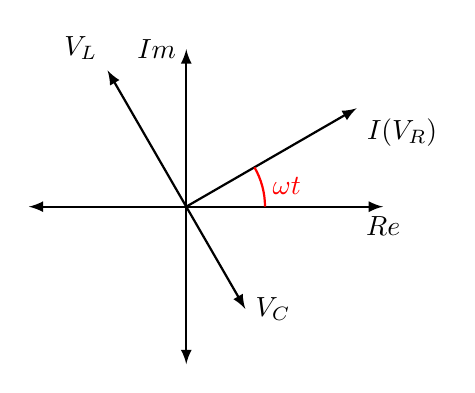
\begin{tikzpicture}[>=latex]
            \draw[style=help lines] (0,0) (3,2);

            \coordinate (vec1) at (300:1.5); 
            \coordinate (vec2) at (30:2.5);
            \coordinate (vec3) at (0:2.5);
            \coordinate (vec4) at (90:2);
            \coordinate (vec5) at (270:2);
            \coordinate (vec6) at (180:2);
            \coordinate (vec7) at (120:2);

            \draw[->,thick,black] (0,0) -- (vec1) node[right] {$V_C$};
            \draw[->,thick,black] (0,0) -- (vec2) node[below right] {$I(V_R)$};
            \draw[->,thick,black] (0,0) -- (vec3) node [below] {$Re$};
            \draw[->,thick,black] (0,0) -- (vec4) node [left] {$Im$};
            \draw[->,thick,black] (0,0) -- (vec5);
            \draw[->,thick,black] (0,0) -- (vec6);
            \draw[->,thick,black] (0,0) -- (vec7) node [above left] {$V_L$};

            \draw [red, thick ] (1.0,0) arc (0:30:1cm)    node [midway, right] {$\omega t$};   
            \end{tikzpicture}

            \end{center}
            \caption{Phase diagram in complex plane} 
        \end{figure}
        The changing current can be seen as a rotating vector in the complex plane, only the projection on the real axis have real world meaning.

        In the complex plane, the reactance of capacitor and inductor is 
        \[
        X_C = \frac{1}{i\omega C} \text{ and } X_L = i\omega L
        \]
    \subsection{AC circuit Problems}
    \subsubsection{AC series circuit with LRC}
    Find the voltage across this circuit when a current of $I = I_0 \sin(\omega t + \phi_0)$ goes through.
        \begin{figure}[H]
            \centering
            \includegraphics[width=10cm]{pics/LRCAC.png}
        \end{figure}
    Through the phase diagram, it is not hard to find $V_{max}$ using vector addition
        \begin{center}
            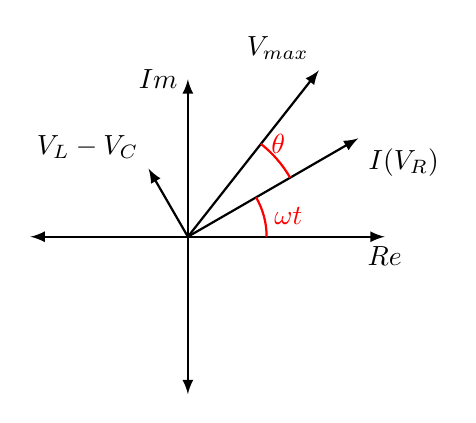
\begin{tikzpicture}[>=latex]
            \draw[style=help lines] (0,0) (3,2);

            \coordinate (vec2) at (30:2.5);
            \coordinate (vec3) at (0:2.5);
            \coordinate (vec4) at (90:2);
            \coordinate (vec5) at (270:2);
            \coordinate (vec6) at (180:2);
            \coordinate (vec7) at (120:1);
            \coordinate (vec8) at (51.8:2.69);

            \draw[->,thick,black] (0,0) -- (vec2) node[below right] {$I(V_R)$};
            \draw[->,thick,black] (0,0) -- (vec3) node [below] {$Re$};
            \draw[->,thick,black] (0,0) -- (vec4) node [left] {$Im$};
            \draw[->,thick,black] (0,0) -- (vec5);
            \draw[->,thick,black] (0,0) -- (vec6);
            \draw[->,thick,black] (0,0) -- (vec7) node [above left] {$V_L-V_C$};
            \draw[->,thick,black] (0,0) -- (vec8) node [above left] {$V_{max}$};            

            \draw [red, thick ] (1.0,0) arc (0:30:1cm)    node [midway, right] {$\omega t$};   
            \draw [red, thick ] ({1.5*cos(30)},{1.5*sin(30)}) arc (30:51.8:1.5cm)    node [right] {$\theta$};   
            \end{tikzpicture}

            \end{center}
        Where $\abs{V_{max}} = \sqrt{(V_L - V_C)^2 + V_R^2}$, all the voltage here are at their maximum, therefore
        \[
            \abs{V_{max}}= \sqrt{\left(\omega L I_0 - \frac{I_0}{\omega C}\right)^2 + I^2_0R^2} = I_0\sqrt{\left(\omega L - \frac{1}{\omega C}\right)^2 + R^2}
        \]
        The projection of $V_{max}$ on the real axis is $V = V_0 \sin(\omega t + \theta)$, where
        \[
            \theta = \arctan{\frac{V_L-V_C}{V_R}} = \arctan{\frac{\omega L - \frac{1}{\omega C}}{R}} = \arctan{\frac{\omega^2 LC - 1}{\omega CR}}
        \]

    \subsubsection{Resonant Circuit}

    \begin{wrapfigure}[14]{r}{2.5cm}
        \includegraphics[width=2.5cm]{pics/ACLRC2.png}
    \end{wrapfigure}

    In the circuit, $L = 0.1$ H, $C = 25\cross 10^{-12}$ F ,$R = 10 \text{ }\Omega$, $U = 50\cross 10^{-3}$ V.
    \begin{enumerate}
        \item Consider the following circuit, at a certain frequency, maximum current will go through this circuit, this is called electrical resonance, find the resonant frequency $f_0$.
        \item Find the voltage arcross inductor when the AC supplys emf at resonant frequency.
    \end{enumerate}

    \textbf{Solution}: 1. The total reactance of this circuit is 
    \[
    X = \sqrt{R^2 + \left(\omega L - \frac{1}{\omega C}\right)^2}
    \]
    The maximum current flows through when the reactance of this circuit hits the minimum, which occurs at $X_C = X_L$
    \begin{align*}
        \omega L &= \frac{1}{\omega C}\\
        (2\pi f_0)^2 &= \frac{1}{LC}\\
        f_0 &= \frac{1}{2\pi\sqrt{LC}}\\
    \end{align*}

    2. When electrical resonant happens, the angular frequency of this circuit is
    \[
    f_0 = \frac{1}{2\pi \sqrt{LC}} = 100658 \text{/s}
    \]
    The voltage across is thus
    \[
    V_L = I Z_L = \frac{U}{R} 2\pi f_0 = 316 \text{ V}
    \]

    \subsubsection{RC RL parallel circuit}
    Consider this circuit, the frequency of AC is $f = 50 $ Hz, each resistor have a equal resistance of $R = 100 \text{ }\Omega$, the reading in each anameter is the same, find the inductance of inductor and capacitance of capacitor.
    \begin{figure}[H]
        \centering
        \includegraphics[width=10cm]{pics/RCRL.png}
    \end{figure}

    \textbf{Solution}:
    Assume one can express the 3 current as a spinning vector in the complex plane. Therefore
    \[
    \vec{I}_1 = \vec{I}_2 + \vec{I}_3
    \]
    Also $I_1 = I_2 = I_3$, which means the three vectors share the same origin but have an angle of $\alpha = 2\pi/3$.
    
    Now consider the phase difference between $I_2$, $I_3$ and voltage, voltage has the same phase as $I_1$, therefore the voltage vector bisects the angle formed by $\vec{I}_2$ and $\vec{I}_3$, which means the phase difference is $\phi = \pi/3$

    This angle can also be expressed from the properties of the circuit
    \[
    \phi_2 = \arctan{\frac{1}{\omega RC}} \text{ and } \phi_3 = \arctan{\frac{\omega L}{R}}
    \]
    Therefore the capacitance of capacitor is 
    \[
    C = \frac{1}{\omega R \tan \phi} = \frac{1}{2\sqrt{3}\pi R f} = 1.838\cross 10^{-5} \text{ F}
    \]
    The inductance of the inductor is
    \[
    L = \frac{R}{\omega} \tan \phi = \frac{\sqrt{3}R}{2\pi f} = 0.551 \text{ H}
    \]
\end{document}